\documentclass[]{article}
\usepackage{lmodern}
\usepackage{amssymb,amsmath}
\usepackage{ifxetex,ifluatex}
\usepackage{fixltx2e} % provides \textsubscript
\ifnum 0\ifxetex 1\fi\ifluatex 1\fi=0 % if pdftex
  \usepackage[T1]{fontenc}
  \usepackage[utf8]{inputenc}
\else % if luatex or xelatex
  \ifxetex
    \usepackage{mathspec}
  \else
    \usepackage{fontspec}
  \fi
  \defaultfontfeatures{Ligatures=TeX,Scale=MatchLowercase}
  \newcommand{\euro}{€}
\fi
% use upquote if available, for straight quotes in verbatim environments
\IfFileExists{upquote.sty}{\usepackage{upquote}}{}
% use microtype if available
\IfFileExists{microtype.sty}{%
\usepackage{microtype}
\UseMicrotypeSet[protrusion]{basicmath} % disable protrusion for tt fonts
}{}
\usepackage[margin=1in]{geometry}
\usepackage{hyperref}
\PassOptionsToPackage{usenames,dvipsnames}{color} % color is loaded by hyperref
\hypersetup{unicode=true,
            pdfborder={0 0 0},
            breaklinks=true}
\urlstyle{same}  % don't use monospace font for urls
\usepackage{color}
\usepackage{fancyvrb}
\newcommand{\VerbBar}{|}
\newcommand{\VERB}{\Verb[commandchars=\\\{\}]}
\DefineVerbatimEnvironment{Highlighting}{Verbatim}{commandchars=\\\{\}}
% Add ',fontsize=\small' for more characters per line
\usepackage{framed}
\definecolor{shadecolor}{RGB}{248,248,248}
\newenvironment{Shaded}{\begin{snugshade}}{\end{snugshade}}
\newcommand{\KeywordTok}[1]{\textcolor[rgb]{0.13,0.29,0.53}{\textbf{{#1}}}}
\newcommand{\DataTypeTok}[1]{\textcolor[rgb]{0.13,0.29,0.53}{{#1}}}
\newcommand{\DecValTok}[1]{\textcolor[rgb]{0.00,0.00,0.81}{{#1}}}
\newcommand{\BaseNTok}[1]{\textcolor[rgb]{0.00,0.00,0.81}{{#1}}}
\newcommand{\FloatTok}[1]{\textcolor[rgb]{0.00,0.00,0.81}{{#1}}}
\newcommand{\ConstantTok}[1]{\textcolor[rgb]{0.00,0.00,0.00}{{#1}}}
\newcommand{\CharTok}[1]{\textcolor[rgb]{0.31,0.60,0.02}{{#1}}}
\newcommand{\SpecialCharTok}[1]{\textcolor[rgb]{0.00,0.00,0.00}{{#1}}}
\newcommand{\StringTok}[1]{\textcolor[rgb]{0.31,0.60,0.02}{{#1}}}
\newcommand{\VerbatimStringTok}[1]{\textcolor[rgb]{0.31,0.60,0.02}{{#1}}}
\newcommand{\SpecialStringTok}[1]{\textcolor[rgb]{0.31,0.60,0.02}{{#1}}}
\newcommand{\ImportTok}[1]{{#1}}
\newcommand{\CommentTok}[1]{\textcolor[rgb]{0.56,0.35,0.01}{\textit{{#1}}}}
\newcommand{\DocumentationTok}[1]{\textcolor[rgb]{0.56,0.35,0.01}{\textbf{\textit{{#1}}}}}
\newcommand{\AnnotationTok}[1]{\textcolor[rgb]{0.56,0.35,0.01}{\textbf{\textit{{#1}}}}}
\newcommand{\CommentVarTok}[1]{\textcolor[rgb]{0.56,0.35,0.01}{\textbf{\textit{{#1}}}}}
\newcommand{\OtherTok}[1]{\textcolor[rgb]{0.56,0.35,0.01}{{#1}}}
\newcommand{\FunctionTok}[1]{\textcolor[rgb]{0.00,0.00,0.00}{{#1}}}
\newcommand{\VariableTok}[1]{\textcolor[rgb]{0.00,0.00,0.00}{{#1}}}
\newcommand{\ControlFlowTok}[1]{\textcolor[rgb]{0.13,0.29,0.53}{\textbf{{#1}}}}
\newcommand{\OperatorTok}[1]{\textcolor[rgb]{0.81,0.36,0.00}{\textbf{{#1}}}}
\newcommand{\BuiltInTok}[1]{{#1}}
\newcommand{\ExtensionTok}[1]{{#1}}
\newcommand{\PreprocessorTok}[1]{\textcolor[rgb]{0.56,0.35,0.01}{\textit{{#1}}}}
\newcommand{\AttributeTok}[1]{\textcolor[rgb]{0.77,0.63,0.00}{{#1}}}
\newcommand{\RegionMarkerTok}[1]{{#1}}
\newcommand{\InformationTok}[1]{\textcolor[rgb]{0.56,0.35,0.01}{\textbf{\textit{{#1}}}}}
\newcommand{\WarningTok}[1]{\textcolor[rgb]{0.56,0.35,0.01}{\textbf{\textit{{#1}}}}}
\newcommand{\AlertTok}[1]{\textcolor[rgb]{0.94,0.16,0.16}{{#1}}}
\newcommand{\ErrorTok}[1]{\textcolor[rgb]{0.64,0.00,0.00}{\textbf{{#1}}}}
\newcommand{\NormalTok}[1]{{#1}}
\usepackage{graphicx,grffile}
\makeatletter
\def\maxwidth{\ifdim\Gin@nat@width>\linewidth\linewidth\else\Gin@nat@width\fi}
\def\maxheight{\ifdim\Gin@nat@height>\textheight\textheight\else\Gin@nat@height\fi}
\makeatother
% Scale images if necessary, so that they will not overflow the page
% margins by default, and it is still possible to overwrite the defaults
% using explicit options in \includegraphics[width, height, ...]{}
\setkeys{Gin}{width=\maxwidth,height=\maxheight,keepaspectratio}
\setlength{\parindent}{0pt}
\setlength{\parskip}{6pt plus 2pt minus 1pt}
\setlength{\emergencystretch}{3em}  % prevent overfull lines
\providecommand{\tightlist}{%
  \setlength{\itemsep}{0pt}\setlength{\parskip}{0pt}}
\setcounter{secnumdepth}{0}

%%% Use protect on footnotes to avoid problems with footnotes in titles
\let\rmarkdownfootnote\footnote%
\def\footnote{\protect\rmarkdownfootnote}

%%% Change title format to be more compact
\usepackage{titling}

% Create subtitle command for use in maketitle
\newcommand{\subtitle}[1]{
  \posttitle{
    \begin{center}\large#1\end{center}
    }
}

\setlength{\droptitle}{-2em}
  \title{}
  \pretitle{\vspace{\droptitle}}
  \posttitle{}
  \author{}
  \preauthor{}\postauthor{}
  \date{}
  \predate{}\postdate{}


% Redefines (sub)paragraphs to behave more like sections
\ifx\paragraph\undefined\else
\let\oldparagraph\paragraph
\renewcommand{\paragraph}[1]{\oldparagraph{#1}\mbox{}}
\fi
\ifx\subparagraph\undefined\else
\let\oldsubparagraph\subparagraph
\renewcommand{\subparagraph}[1]{\oldsubparagraph{#1}\mbox{}}
\fi

\usepackage{ctex} 
\setCJKmainfont{宋体}                     % 中文缺省字体,
\setCJKsansfont{黑体}                      % 中文无衬线字体,   调用命令: \sffamily
\setCJKmonofont{仿宋}     % 中文打字机(等宽)字体, 调用命令: \ttfamily

%\usepackage{ctex} 
%\setCJKmainfont{Adobe 宋体 Std}                     % 中文缺省字体,
%\setCJKsansfont{Adobe 黑体 Std}                      % 中文无衬线字体,   调用命令: \sffamily
%\setCJKmonofont{Adobe 仿宋 Std}     % 中文打字机(等宽)字体, 调用命令: \ttfamily

\begin{document}

\section{\texorpdfstring{\textbf{5.}}{5.}}\label{section}

\subsection{R code:}\label{r-code}

\begin{Shaded}
\begin{Highlighting}[]
\KeywordTok{library}\NormalTok{(ggplot2)}
\NormalTok{norm_distribution<-function(num)}
\NormalTok{\{}
  \KeywordTok{rnorm}\NormalTok{(num,}\DecValTok{0}\NormalTok{,}\DecValTok{1}\NormalTok{)}
\NormalTok{\}}

\NormalTok{chisq_distribution<-function(num)}
\NormalTok{\{}
  \KeywordTok{rchisq}\NormalTok{(num,}\DecValTok{12}\NormalTok{)}
\NormalTok{\}}

\NormalTok{inverse_chisq_distribution<-function(num)}
\NormalTok{\{}
  \DecValTok{1}\NormalTok{/(}\KeywordTok{rchisq}\NormalTok{(num,}\DecValTok{12}\NormalTok{))}
\NormalTok{\}}

\NormalTok{cauchy_distribution<-function(num)}
\NormalTok{\{}
  \KeywordTok{rcauchy}\NormalTok{(num)}
\NormalTok{\}}

\NormalTok{x_bar_plot<-function(func)}
\NormalTok{\{}
  \NormalTok{n<-}\KeywordTok{seq}\NormalTok{(}\DecValTok{100}\NormalTok{,}\DecValTok{1000}\NormalTok{,}\DecValTok{100}\NormalTok{)}
  \KeywordTok{set.seed}\NormalTok{(}\DecValTok{520}\NormalTok{)}
  \NormalTok{x<-}\KeywordTok{sapply}\NormalTok{(n, func)}
  \NormalTok{x_bar<-}\KeywordTok{sapply}\NormalTok{(x, mean)}
  \CommentTok{#print(paste0("mean of x_bar=",mean(x_bar)))}
  \NormalTok{q<-}\KeywordTok{qplot}\NormalTok{(n,x_bar)}
  \NormalTok{q+}\KeywordTok{scale_x_continuous}\NormalTok{(}\DataTypeTok{breaks =} \NormalTok{n)}
\NormalTok{\}}
\end{Highlighting}
\end{Shaded}

\newpage

\subsection{(a)}\label{a}

\begin{Shaded}
\begin{Highlighting}[]
\KeywordTok{x_bar_plot}\NormalTok{(norm_distribution)}
\end{Highlighting}
\end{Shaded}

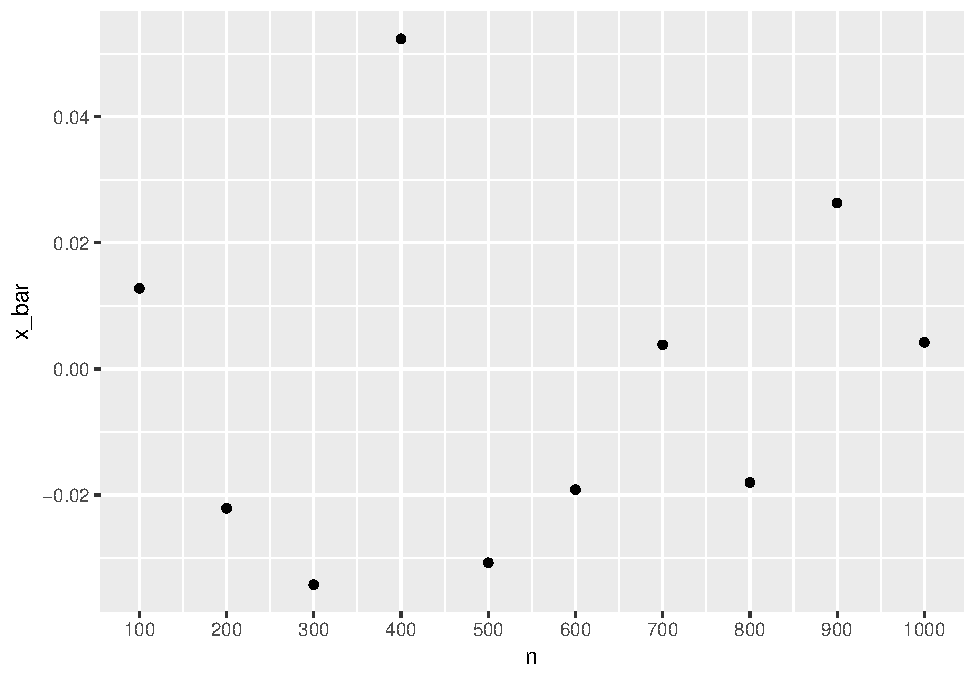
\includegraphics{advEconometric_homework_files/figure-latex/unnamed-chunk-2-1.pdf}

\subsubsection{conclusion:}\label{conclusion}

\subsubsection{1.x\_bar围绕分布的期望EX=0.00波动。}\label{xux5fbarex0.00}

\subsubsection{2.x\_bar与sample size 没有必然联系,并不存在sample size
越大,x\_bar越接近于EX。同时可用n=1000,2000\ldots{}10000验证。}\label{xux5fbarsample-size-sample-size-xux5fbarexn1000200010000}

 \newpage

\subsection{(b)}\label{b}

\begin{Shaded}
\begin{Highlighting}[]
\KeywordTok{x_bar_plot}\NormalTok{(chisq_distribution)}
\end{Highlighting}
\end{Shaded}

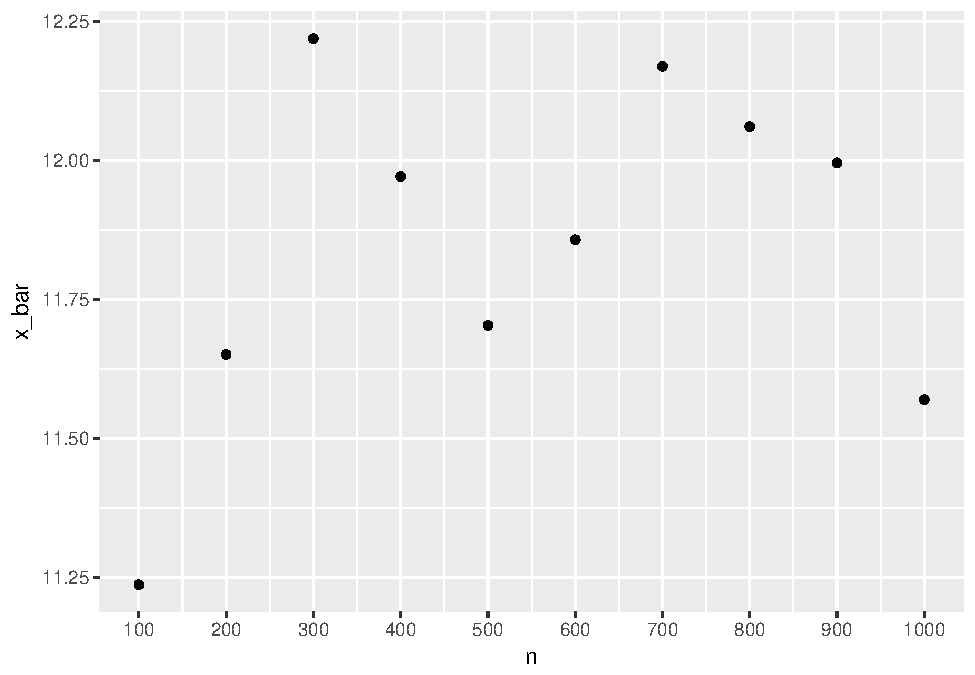
\includegraphics{advEconometric_homework_files/figure-latex/unnamed-chunk-3-1.pdf}

\subsubsection{conclusion:}\label{conclusion-1}

\subsubsection{1.x\_bar围绕分布的期望EX=12波动。}\label{xux5fbarex12}

\subsubsection{2.x\_bar与sample size 没有必然联系,并不存在sample size
越大,x\_bar越接近于EX。}\label{xux5fbarsample-size-sample-size-xux5fbarex}

 \newpage

\subsection{(c)}\label{c}

\begin{Shaded}
\begin{Highlighting}[]
\KeywordTok{x_bar_plot}\NormalTok{(inverse_chisq_distribution)}
\end{Highlighting}
\end{Shaded}

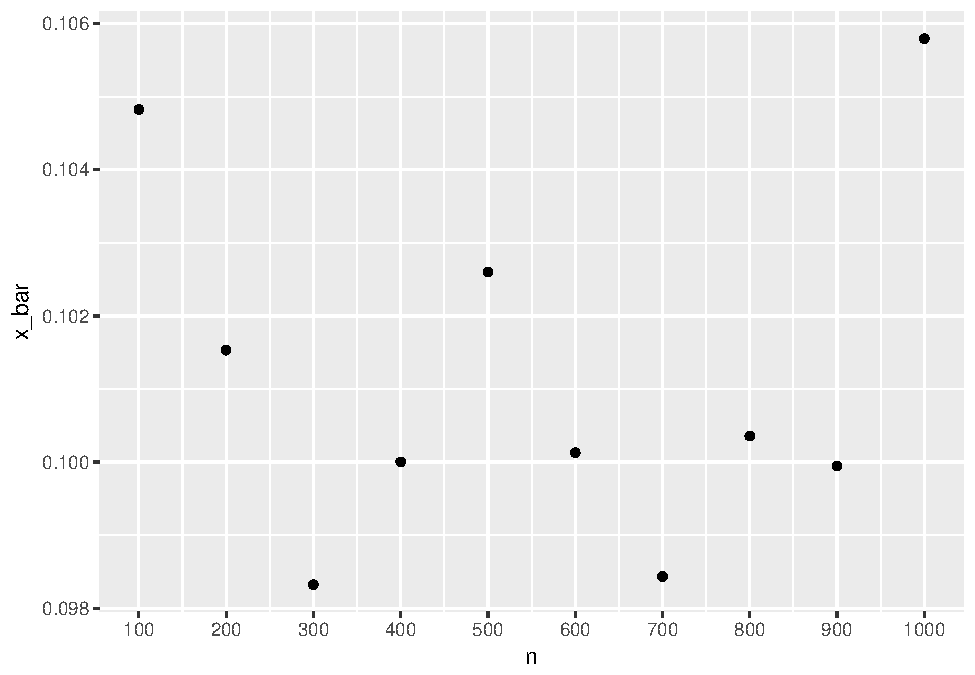
\includegraphics{advEconometric_homework_files/figure-latex/unnamed-chunk-4-1.pdf}

\subsubsection{conclusion:}\label{conclusion-2}

\subsubsection{1.x\_bar围绕0.1波动。}\label{xux5fbar0.1}

\subsubsection{2.x\_bar与sample size 没有必然联系,并不存在sample size
越大,x\_bar越接近于0.1。}\label{xux5fbarsample-size-sample-size-xux5fbar0.1}

 \newpage

\subsection{(d)}\label{d}

\begin{Shaded}
\begin{Highlighting}[]
\KeywordTok{x_bar_plot}\NormalTok{(cauchy_distribution)}
\end{Highlighting}
\end{Shaded}

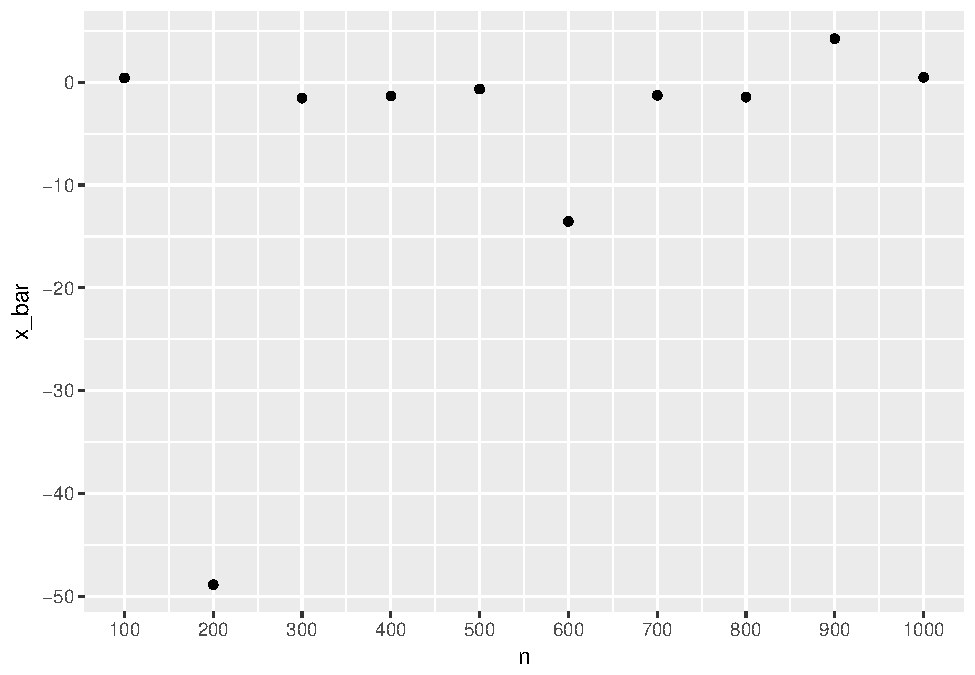
\includegraphics{advEconometric_homework_files/figure-latex/unnamed-chunk-5-1.pdf}

\subsubsection{conclusion:}\label{conclusion-3}

\subsubsection{1.x\_bar围绕0.00波动,大多数点波动范围非常小,近乎接近于0.00。但是个别点与0.00偏差很大。}\label{xux5fbar0.000.000.00}

\subsubsection{2.x\_bar与sample size 没有必然联系,并不存在sample size
越大,x\_bar越接近于0.00。}\label{xux5fbarsample-size-sample-size-xux5fbar0.00}

\end{document}
